\capitulo{5}{Aspectos relevantes del desarrollo del proyecto}

En este apartado se recogen los aspectos más importantes o relevantes del desarrollo del proyecto. Desde las decisiones tomadas hasta las implicaciones que conlleva. Además de los problemas que fueron surgiendo durante todo el proceso.

\section{Comienzo del trabajo final de grado}
La idea de mi proyecto, surge de la noche a la mañana, porque era día 20 de junio y no tenía nada para entregar. Esto se debía a que inicialmente iba a hacer otro proyecto basado en \emph{Knime}.

No podía dejar pasar una convocatoria más. El otro proyecto no me motivaba lo suficiente y tenía poca documentación al respecto. Aparte no me sentía cómodo con el tema, ya que la situación de emergencia sanitaria que hemos pasado estos meses, no ha ayudado precisamente a tener buen ánimo.

Por lo que decidí estudiar cómo estaba el mercado de la programación móvil, descubriendo Flutter. Me gustó mucho que todo lo que se comentaba sobre este \emph{Framework}, eran cosas buenas, era algo novedoso y sobretodo lo que más me decantó a cogerlo fue el respaldo que le da Google.

Esto se lo comenté a mis tutores de trabajo final de grado, dándome el visto bueno, pero debía trabajar mucho para llegar a la calidad esperada. Por lo que era un reto enorme al que me enfrentaba, pero como digo, no se pueden dejar pasar las oportunidades. Por otra parte lo que más me incentivaba, era que a la hora de buscar trabajo, no podía acreditar mi titulación como ingeniero, por lo que el trabajo final de grado es el último paso que se debe de completar, antes de encontrar empleo.

Ya que muchas de las empresas me decían que me esperaban a que terminase, para luego cogerme. Y yo no podía esperar, porque si no hacía el TFG, debía de trabajar para no tener que pensar en esto. Por lo que me encontraba entre la <<espada y la pared>>.

En definitiva me siento muy agradecido a mis tutores, por haberme dejado cambiar de proyecto, por animarme a conseguirlo, por el feedback constante y darme el soporte necesario.

Al final la idea fue la de realizar una aplicación móvil para Android con Flutter, que consistía en una colección de videojuegos, de los que la base inicial sería el snake y el cuatro en raya online. Con publicidad, para obtener rendimiento económico o un ranking donde mostrar el mejor jugador del snake.

\section{Proceso de aprendizaje y búsqueda de información}
Al comienzo del proyecto mi idea sobre este lenguaje de programación era nula, para ello fue necesario realizar un curso en ~\href{https://www.udemy.com/course/flutter-primeros-pasos/}{Udemy}, de unas 40 horas en dos días y medio, para conocer los elementos más básicos de Dart y Flutter.

Una vez con las nociones necesarias para arrancar el proyecto, la primera fuente de donde extraje la información fue la API de Flutter, que se encuentra en su página web~\cite{google:apiflutter}. Aquí se pueden encontrar la documentación de cada uno de los Widgets, pero también algunos tutoriales sobre como desplegar la aplicación, como integrarlo con otras plataformas o sistemas.

Desde la web anterior también se nos indica la referencia a muchos de los paquetes que crea al comunidad~\cite{google:pubdev}.


\section{Flutter es asíncrono}
Uno de los mayores retos cuando empiezas a trabajar con este \emph{framework} es que se trabaja de manera asíncrona. Durante el curso estos aspectos se ven de una manera muy básica, por lo que fue necesario una mayor documentación al respecto.

Es decir, todo la aplicación se ejecuta en un único hilo, por lo que si un bloque de código se queda congelado, se cuelga todo el programa. Entonces surgen las operaciones asíncronas, que permiten crear funciones o fragmentos de código que no detengan la aplicación entera, porque estas se ejecutan en otros hilos. Ya que para algunas situaciones es necesario quedarse a la espera, como puede ser la llegada de datos de un servidor muy lejano, por lo que no se puede dar al cliente la sensación de que la aplicación se a congelado y no responde.

Dentro de Dart son los llamados \verb|Future<Object>|. Básicamente son tareas que se quedan a la espera, con el fin de que se las devuelva el objeto pedido. Un ejemplo de esto lo podemos ver en la figura~\ref{fig:future}.

\begin{figure}[H]
	\centering
	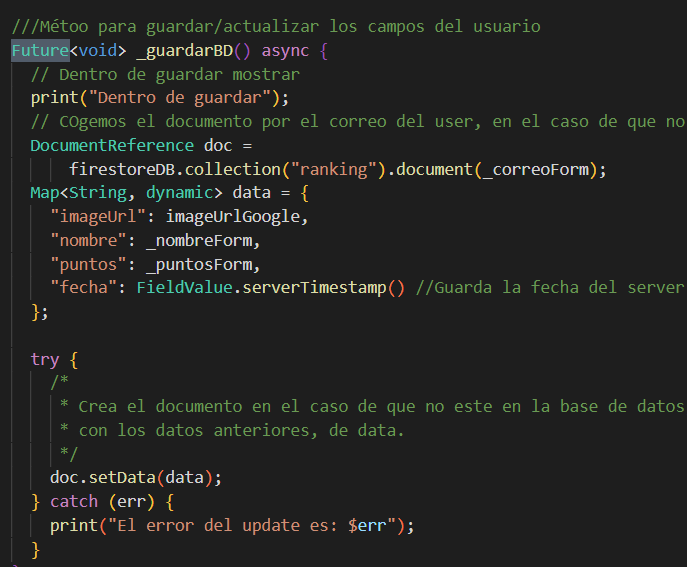
\includegraphics[width=1\textwidth]{teoria/future.png}
	\caption{Ejemplo de Future}\label{fig:future}
\end{figure}

Para ello tenemos que declarar las funciones que son asíncronas con la palabra reservada \texttt{async}, de tal manera que devolverá los resultados en un tiempo $x$.

Cuando realicemos la llamada a estas funciones, indicaremos que se queden a la espera de respuesta con la palabra reservada del lenguaje \texttt{await}.

Pero podemos encontrarnos con otros objetos que también manejan tareas futuras, como es el caso de los \texttt{Stream}. Haciendo que la aplicación de flutter sea reactiva, como cuatro en raya o el ranking del snake.

Que una aplicación tenga \texttt{Stream} significa que esta se queda a la escucha de cambios de los datos. Estos generalmente se encuentran en un servidor. En el momento en el que se produzca un cambio de estos datos, desencadenará un evento del \texttt{Stream} para actualizar las variables locales.
Para que esta sea reactiva, los datos del \texttt{Stream} tienen que estar en el \texttt{builder}, de tal manera que la interfaz de usuario se va a rediseñar por cada cambio.

%\section{Nuevas formas de hacer if}
%Desconocía totalmente esta nueva forma de hacer los condicionales, ya que deja un código más limpio, que ocupa menos líneas e intuitivo. Un ejemplo de esto se puede ver en la imagen siguiente~\ref{fig:nuevoif}:
%
%\begin{figure}[H]
%	\centering
%	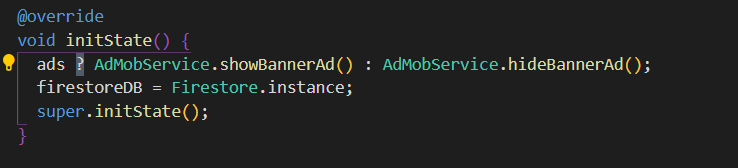
\includegraphics[width=1\textwidth]{teoria/nuevoif.png}
%	\caption{Nuevas formas if}\label{fig:nuevoif}
%\end{figure}

\section{Play Store}
Uno de los problemas encontrados fue a la hora de tener que generar las claves de seguridad, para que la aplicación se pueda subir a la tienda y que ciertos de los servicios estén operativos.

La incidencia se producía cuando generaba las claves, debido a que estaba usando la clave para \emph{debug} y no para \emph{release}, imposibilitando la subida, por el control que hace la tienda de las aplicaciones que se suben.

Esto era debido a que en la documentación de Flutter siempre se realiza para el modo de test. Luego otra de las cosas a vigilar, es la ruta donde dejamos la clave y la configuración de algunos de los ficheros, como los \emph{.gradle} o el manifest.

También es fundamental tener la clave bien guardada porque en el caso de que se pierda, vamos a tener que volver a realizar el proceso desde cero y se convertiría en algo tedioso.

\section{AdMob}
Otro de los problemas que se me presentaron fue cuando pretendía mostrar los anuncios en la aplicación, ya que solo me dejaba usar los anuncios de test que me proporciona Google Ad. He revisado cada uno de los Ids, como se puede ver en la figura~\ref{fig:idbanner}, pero no lo he conseguido.

\begin{figure}%[H]
	\centering
	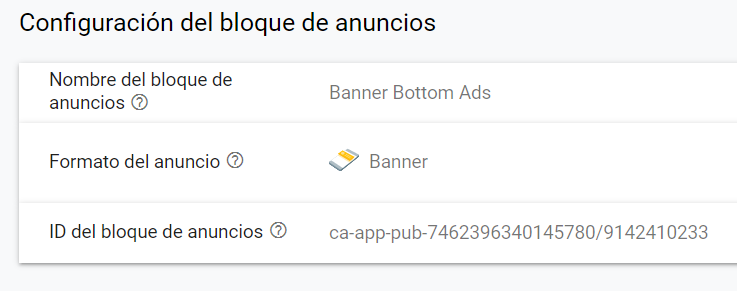
\includegraphics[width=1\textwidth]{teoria/idbanner.png}
	\caption{Banner}\label{fig:idbanner}
\end{figure}

Y las métricas de usuario si que funcionan, ver figura~\ref{fig:metricas}, lo que indica que la instancia de adMob es la correcta.

\begin{figure}%[H]
	\centering
	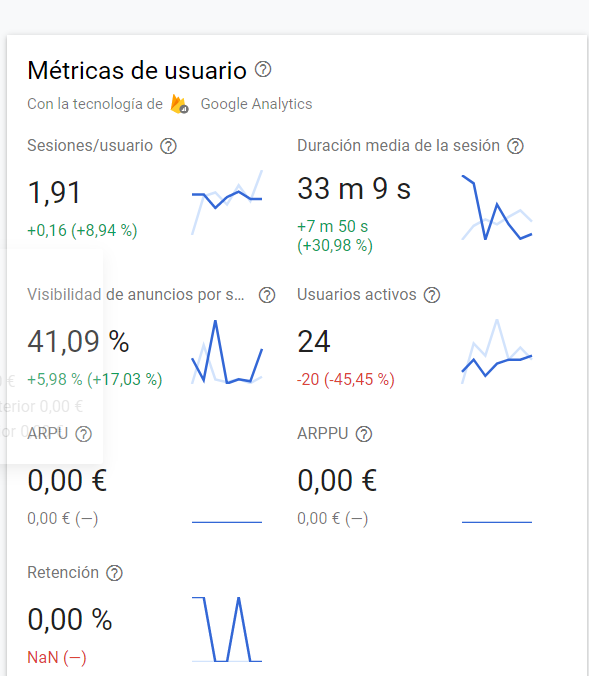
\includegraphics[height=0.8\textwidth]{teoria/metricas.png}
	\caption{Métricas usuarios}\label{fig:metricas}
\end{figure}

Tras investigar y realizar gran cantidad de pruebas creo que el problema puede estar en que no tengo métodos de cobro de ingresos. Por lo tanto la propia Google ni se molesta en poner anuncios. Pero es que la propia consola web de admob, no me deja introducir un método de pago, como se puede ver en la figura~\ref{fig:pagos}:

\begin{figure}%[H]
	\centering
	
\includegraphics[width=1\textwidth]{teoria/pagos.png}
	\caption{Pagos adMob no van}\label{fig:pagos}
\end{figure}



